% Notes de cours pour ACT-2005
% Automne 2018
\documentclass[12pt, french]{report}

% Lien vers un template de préambule
% !TEX encoding = UTF-8 Unicode
% LaTeX Preamble
% Author : Gabriel Crépeault-Cauchon
% Last update : 08/09/2019
% ---------------------------------------------
% BEGINNING OF PREAMBLE
% ---------------------------------------------
% Encoding packages
\usepackage[utf8]{inputenc}
\usepackage[T1]{fontenc}
\usepackage{babel}
\usepackage{lmodern}

% HYPERREF (URL's and Link options)
\usepackage{hyperref}
\hypersetup{colorlinks = true, urlcolor = red!60!black, linkcolor = red!60!black}

% POLICY (choose one of them)
%	\usepackage{concrete}
%	\usepackage{mathpazo}
%	\usepackage{frcursive} %% permet d'écrire en lettres attachées
 \usepackage{aeguill}
% 	\usepackage{mathptmx}
%	\usepackage{fourier} 

% Mathematics configuration
\usepackage{amsmath,amsthm,amssymb,latexsym,amsfonts}
\usepackage{empheq}
\usepackage{numprint}
\usepackage{dsfont} 


% Tcolorbox config
\usepackage{tcolorbox}
\tcbuselibrary{xparse}
\tcbuselibrary{breakable}

% Définition Boite pour exemple
\newcounter{ex}[section]
\DeclareTColorBox{exemple}{ o }% #1 parameter
{colframe=green!20!black,colback=green!5!white, % color of the box
breakable, pad at break*=0mm, % to split the box
before title = {\textbf{Exemple \stepcounter{ex} \arabic{chapter}.\arabic{section}.\arabic{ex} }},
IfValueTF = {#1}{title= {#1}}{title= \hphantom},
after title = {\large \hfill \faWrench}
}

%% Définition boite pour définition
\newcounter{def}[section]
\DeclareTColorBox{definition}{ o }% #1 parameter
{colframe=blue!60!green,colback=blue!5!white, % color of the box
breakable, pad at break*=0mm, % to split the box
before title = {\textbf{Définition \stepcounter{def} \arabic{chapter}.\arabic{section}.\arabic{def} }},
title = {#1},
after title = {\large \hfill \faBook}
}

\DeclareTColorBox{note}{ o }
    {colframe=black,
     colback=white,
     sharp corners,
     pad at break*=0mm,
     IfValueTF={#1}{title={#1}, fonttitle=\bfseries}{title=Note, fonttitle=\bfseries}}


% Graphics and picture import Packages
\usepackage{graphicx}
\usepackage{pict2e}

% insert PDF package
\usepackage{pdfpages}

% Color package
\usepackage{color, soulutf8, colortbl}

% Mathematics table
\usepackage{array}   % for \newcolumntype macro
\newcolumntype{L}{>{$}l<{$}} % math-mode version of "l" column type

% usefull shortcut for colored text
\newcommand{\orange}{\textcolor{orange}}
\newcommand{\red}{\textcolor{red}}
\newcommand{\cyan}{\textcolor{cyan}}
\newcommand{\blue}{\textcolor{blue}}
\newcommand{\green}{\textcolor{green}}
\newcommand{\darkgreen}{\textcolor{darkgreen}}
\newcommand{\purple}{\textcolor{magenta}}
\newcommand{\yellow}{\textcolor{yellow}}

% Colors define
\definecolor{darkgreen}{RGB}{37, 128, 40}
\definecolor{tocColor}{HTML}{8A2507}

% Custum enumerate & itemize Package
\usepackage{enumitem}
% French Setup for itemize function
\frenchbsetup{StandardItemLabels=true}

% Mathematics shortcut
\usepackage{cancel}
\newcommand{\reels}{\mathbb{R}}
\newcommand{\entiers}{\mathbb{Z}}
\newcommand{\naturels}{\mathbb{N}}
\newcommand{\eval}{\biggr \rvert}
\newcommand{\esp}[1]{\mathrm{E} \left[ #1 \right]} % espérance
\newcommand{\variance}[1]{\mathrm{Var} \left( #1 \right)} % variance
\newcommand{\covar}[1]{\mathrm{Cov} \left( #1 \right)} % variance
\newcommand{\prob}[1]{\Pr \left( #1 \right)} % probabilité entre parenthèses
\newcommand{\laplace}{\mathcal{L}}
\newcommand{\matr}[1]{\mathbf{#1}} % Notation matricielle
\DeclareMathOperator{\Tr}{Tr}
\newcommand{\fgp}{\mathcal{P}}
\DeclareMathOperator{\Adj}{Adj}
\newcommand{\derivee}[1]{\frac{\partial}{\partial #1}}
\newcommand{\indic}[1]{\mathds{1}_{\{ #1 \}}}
\newcommand{\VaR}[2][k]{\mathrm{VaR}_{#1}{\left( #2 \right)}}
\newcommand{\TVaR}[2][k]{\mathrm{TVaR}_{#1}{\left( #2 \right)}}


% Matricial anotation for math symbols (\bm{•})
% à enlever éventuellement, j'ai ajouté la macro \matr{} à la place.
\usepackage{bm}

% Actuarial notation package
\usepackage{actuarialsymbol}
\usepackage{actuarialangle}

% To indicate equation number on a specific line in align environment
\newcommand\numberthis{\addtocounter{equation}{1}\tag{\theequation}}

% Other shortcut
\newcommand{\p}{\paragraph{}}
\newcommand{\n}{\newline}

% source : https://tex.stackexchange.com/questions/112576/math-mode-in-tabular-without-having-to-use-everywhere



% Special symbols package
 \usepackage[tikz]{bclogo}
\usepackage{fontawesome}

% Retire l'indentation automatique de Latex
\setlength{\parindent}{0pt}

% Utilisé pour la page couverture
\usepackage[absolute]{textpos} % Textblock environement
\usepackage{anyfontsize} % Avoir un gros titre
\usepackage{titling} % Avoir un gros titre
\usepackage{changepage} % ajustwidth environement

% Pour afficher du code
\usepackage{listings}

\definecolor{codegray}{gray}{0.9}
\newcommand{\code}[1]{\colorbox{codegray}{\texttt{#1}}}

\definecolor{insideBlackTerminal}{RGB}{33,33,33}
% Set Language
% \lstset{
%     language={bash},
%     basicstyle=\small\ttfamily\color{white}, % Global Code Style
%     captionpos=b, % Position of the Caption (t for top, b for bottom)
%     extendedchars=true, % Allows 256 instead of 128 ASCII characters
%     tabsize=2, % number of spaces indented when discovering a tab 
%     columns=fixed, % make all characters equal width
%     keepspaces=true, % does not ignore spaces to fit width, convert tabs to spaces
%     showstringspaces=false, % lets spaces in strings appear as real spaces
%     breaklines=true, % wrap lines if they don't fit
%     frame=single, % draw a frame at the top, right, left and bottom of the listing
%     numberstyle=\tiny\ttfamily, % style of the line numbers
%     % commentstyle=\color{red}, % style of comments
%     % keywordstyle=\color{red}, % style of keywords
%     % stringstyle=\color{red}, % style of strings
%     backgroundcolor = \color{insideBlackTerminal},
%     rulecolor=\color{red}
% }

\usepackage{lstlinebgrd}
\definecolor{grayComment}{HTML}{8D90B8}
\lstset{
language=R,                     % the language of the code
basicstyle=\ttfamily, % the size of the fonts that are used for the code
% numbers=left,                   % where to put the line-numbers
% numberstyle=\color{blue},  % the style that is used for the line-numbers
% stepnumber=1,                   % the step between two line-numbers. If it is 1, each line
% will be numbered
numbersep=5pt,                  % how far the line-numbers are from the code
backgroundcolor=\color{white},  % choose the background color. You must add \usepackage{color}
linebackgroundcolor=\color{white},
showspaces=false,               % show spaces adding particular underscores
showstringspaces=false,         % underline spaces within strings
showtabs=false,                 % show tabs within strings adding particular underscores
frame=single,                   % adds a frame around the code
rulecolor=\color{black},        % if not set, the frame-color may be changed on line-breaks within not-black text (e.g. commens (green here))
tabsize=2,                      % sets default tabsize to 2 spaces
captionpos=b,                   % sets the caption-position to bottom
breaklines=true,                % sets automatic line breaking
breakatwhitespace=false,        % sets if automatic breaks should only happen at whitespace
%   keywordstyle=\color{functionR},      % keyword style
commentstyle=\color[HTML]{9F0808},  %\color[HTML]{8D90B8},   % comment style
%   stringstyle=\color[HTML]{1D9507},      % string literal style
moredelim=**[is][\color{grayComment}]{@}{@}, % couleur manuel
literate=%
{à}{{\`a}}1
{é}{{\'e}}1
{è}{{\`e}}1
} 




















































% ---------------------------------------------
% END OF PREAMBLE
% ---------------------------------------------

%% Preamble for code listing
% Please input this file after your main preamble
% Gabriel Crépeault-Cauchon, 2018
% -------------------------------

% Load the package 
\usepackage{listings}

% -------
% Settings for different programming language : 

% VISUAL BASIC FOR APPLICATION (VBA)
\lstdefinestyle{vba}
{
	language = {[Visual] Basic},	
	breaklines = true,
	extendedchars=\true,
	showstringspaces = false,	
	tabsize = 3,
	breaklines = true,
	keywordstyle = \color{blue},
	commentstyle = \color{green!35!black},
	backgroundcolor = \color{gray!20!white},
	stringstyle = \color{red}
}


% R (to be modified : does not work for now.
\lstdefinestyle{SAS}
{
	language=SAS
}




% Information sur le document
\title{Mathématiques actuarielles IARD-1 \\
ACT-2005 \\
Notes de cours}
\author{Gabriel Crépeault-Cauchon \\
Nicholas Langevin}


% -----------------------------------
% --- DÉBUT DU DOCUMENT ---
\begin{document}

% Page titre
\maketitle

% Table des matières
\tableofcontents

% --- DÉBUT DE LA RÉDACTION ---

% --- RÉSUMÉ ---
\begin{abstract}
Ce document résume les notes de cours prises en classe dans le cours de Mathématiques actuarielles IARD-1, ainsi que des notions prises du livre \textit{LOSS MODELS - From Data to Decisions, 4\up{th} edition}.
\end{abstract}
% --------------


\setcounter{chapter}{2} % Pour aller directement au chapitre 3
\chapter{Quantités des distributions à connaître}
\section{Moments}

\paragraph{\textit{Raw moments}}
On représente le $k$\up{e} moment par $\mu_k^\prime$, soit
\begin{equation}
\mu_k^\prime = \esp{X^k} 
\end{equation}

\paragraph{Moments centraux} Le $k$\up{e} moment central est représenté par
\begin{equation}
\mu_k = \esp{(X - \mu)^k}
\end{equation}

\begin{exemple}[Quelques exemples de moments centraux]
La variance est le 2\up{e} moment central : 
\begin{align*}
Var(X) = \mu_2 =  \esp{(X - \mu)^2} \\
\end{align*}
Le 3\up{e} moment centré, qui est utilisé pour calculer le coefficient d'asymétrie : 
\begin{align*}
\mu_3 = \esp{(X-\mu)^3}
\end{align*}
\end{exemple}

\paragraph{Coefficient de variation}
\begin{equation}
CV = \frac{\sigma}{\esp{X}}
\end{equation}


\paragraph{Coefficient d'asymétrie}
Le coefficient d'asymétrie, aussi appelé \textit{skewness}, est défini par
% J'ai pris la notation du livre Loss Model pour le skewness.
\begin{equation}
\gamma_1 = \frac{\mu_3}{\sigma^3}
\end{equation}
Soit le 3\up{e} moment standarisé. Si $S_k = 0$, alors la distribution tend vers une loi normale, telle qu'on le voit sur la figure ci-dessous : 

\begin{center}
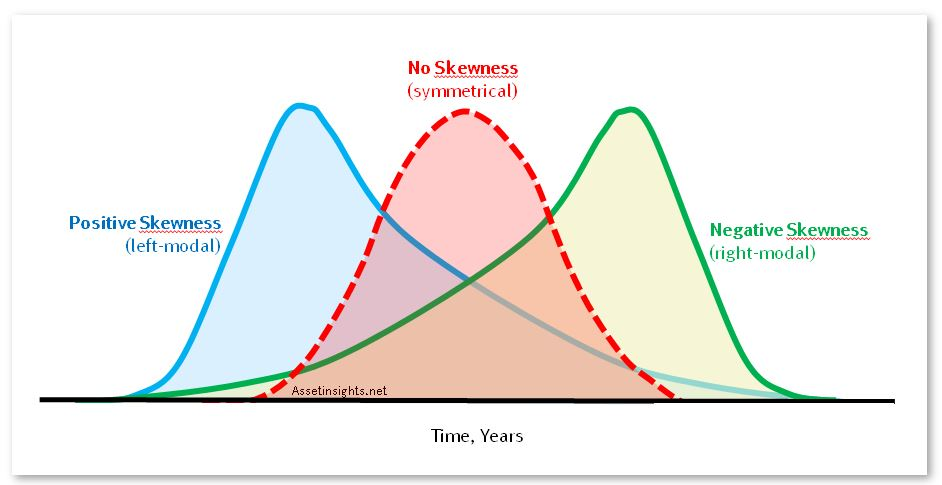
\includegraphics[scale=0.4]{../MAS-I/src/skewness_interpretation.jpg}
\end{center}

\paragraph{Coefficient d'applatissement}
Le coefficient d'applatissement, aussi appelé \textit{Kurtosis}, se définit par
\begin{equation}
\text{Kurtosis} = \frac{\mu_4}{\sigma^4}
\end{equation}
Cette quantité permet de mesurer l'épaisseur de l'aile (\textit{tail}) de la distribution. Si $\esp{z^4} =3$, alors la distribution tend vers une loi normale $N(\mu, \sigma^2)$.

\paragraph{Mean Excess Loss}
On définit la variable aléatoire $Y^P$, qui représente le montant de perte en excès d'un déductible $d$, sachant que la perte est au delà de ce montant. On peut définir l'espérance des coûts de cette variable alétaoire : 
\begin{equation}
e(d) = \esp{Y^P} = \esp{X-d | X \geq d} = \frac{\int_{d}^{\infty} S_X(x)}{S_X(d)}
\end{equation}

Note : cette variable est dite tronquée à gauche et \textit{shifted}. On entend parfois aussi \textit{Per-payment}
	

\paragraph{Left censored and shifted variable}
Soit la v.a. $Y^L$, qui représente le montant payé par l'assureur \textit{par perte}. La variable est donc dite \textit{censurée à gauche et shifted}. On peut aussi en calculer l'espérance : 
\begin{equation}
\esp{Y^L} = \esp{(X-d)_+} = \int_{d}^{\infty} (x-d) f_X(x) dx
\end{equation}
De plus, on peut facilement déduire la relation suivante : 
\begin{align*}
\esp{(X-d)_+} = e(d) (1 - F_X(d))
\end{align*}

\paragraph{Limited Loss Variable} Finalement, on peut définir la variable $Y$, qui représente le paiement de l'assureur avec une limite de $u$ à la police. Son espérance est définie par
\begin{equation}
\esp{X \wedge u} = \int_{0}^{u} f_X(x) dx
\end{equation}
À l'aide d'intégration par partie, on peut trouver la forme suivante : 
\begin{align*}
\esp{X \wedge u} = \int_{0}^{u} S_X(x) dx
\end{align*}
La v.a. $Y$ est dite \textit{censurée à droite et shifted}

\begin{exemple}[lien entre le déductible et la limite]
On peut faire le lien entre le déductible et la limite : 
\begin{center}
%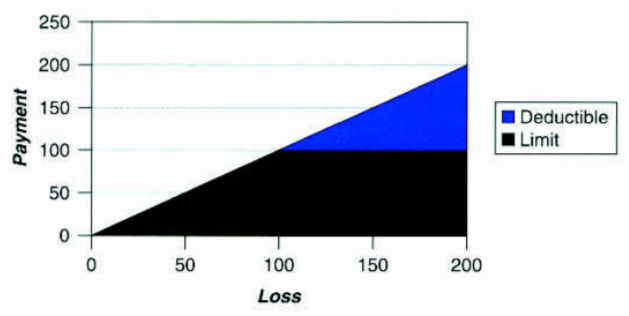
\includegraphics[scale=0.45]{../MAS-I/src/distinction_loss-deductible-limit}
\end{center}
\end{exemple}

\setcounter{section}{3}
% Ne semble pas pertinent pour l'Examen ...
%\section{La loi normale}
%
%\paragraph{La fonction génératrice des moments}
%\begin{align*}
%    M_x(t) &= M_x(0) + \frac{M_x^\prime t}{1!} + \frac{M_x^{\prime\prime} t^2}{2!} + ... + \frac{M_x^{(n) t^n}}{n!} \\
%           &= 1 + \frac{E[x] t}{1!} + \frac{E[x^2] t^2}{2!} + ... + \frac{E[x^n] t^n}{n!}
%\end{align*}
%
%On pose: $c_k = \frac{E[x^n]}{n!}$ alors,
%
%\begin{equation}
%    E[x^k] = C_k k!
%\end{equation}

\section{Queue de distribution}
\subsection{Classification selon les moments}
\begin{enumerate}[label=\faAngleRight]
\item On peut déterminer si une distribution a une \textit{heavy-tail} en vérifiant si ses moments existent.

\item On peut aussi comparer des distributions entre-eux en utilisant des quantités standarisées, telles que le Coefficient de variation, le coefficient d'asymétrie (\textit{skewness}) ou encore le coefficient d'applatissement (\textit{Kurtosis})
\end{enumerate}

\subsection{Classification selon les comportements limites des ailes de distribution}
\begin{enumerate}[label=\faAngleRight]
\item On peut faire le ratio de deux distributions avec leurs fonction de survie ($S(x)$) ou leur fonction $f$ de densité pour vérifier laquelle des 2 a la plus grosse aile de distribution (\textit{tail}).

\end{enumerate}

\begin{enumerate}
    \item Sois $f_1(x)$ une fonction tels que les 3 premiers moment existe: $E[x^4] = \infty$
    \item Sois $f_2(x)$ une fonction tels que les 2 premiers moment existe: $E[x^2] = \infty$
\end{enumerate}
Alors,
\begin{align*}
    \lim_{x\to\infty} r(x) = \frac{f_1(x)}{f_2(x)} = \left\{
                                                        \begin{array}{ll}
                                                            \infty ,\: f_1(x) \text{a une aile plus lourde que} f_2(x) \\
                                                            0      ,\: f_2(x) \text{a une aile plus lourde que} f_1(x) 
                                                        \end{array}
                                                    \right.
\end{align*}
\begin{exemple}
    Sois $f_{x_1}(x_1) \sim pareto(\alpha, \theta)$ et $f_{x_2}(x_2) \sim gamma(\alpha, \lambda)$ 
    \begin{align*}
        \lim_{x\to\infty} r(x) &= \lim_{x\to\infty} \frac{f_{x_1}(x_1)}{f_{x_2}(x_2)} \\
                               &= \frac{\frac{\alpha \theta^\alpha}{(x + \theta)^{\alpha + 1}}}{\lambda^\alpha x^{\alpha - 1} e^{-\lambda x}} \\
                               &= C \frac{e^{-\lambda x}}{x^{\alpha - 1} (x + \theta)^{\alpha + 1}} \\
                               &= \infty
    \end{align*}      
    La pareto a une queue plus lourde que la gamma
\end{exemple}


\subsection{Classification basée sur la fonction de Hazard}

\begin{definition}[\textit{Hazard rate function}]
La fonction de hazard (aussi appelée force de mortalité ($\mu(x)$) ou le failure rate ($\lambda(x)$), est définie par
\begin{equation}
h_X(x) = \frac{f_X(x)}{S_X(x)}
\end{equation}
On peut aussi exprimer la fonction $h_X(x)$ comme
\begin{align*}
h_X(x) = - \ln (S_X(x))
\end{align*}
\end{definition}
Soit une distribution ayant fonction de densité $f_X(x)$ et fonction de hazard $h_X(x)$. Alors,
\begin{enumerate}[label=\faAngleRight]
\item Si $h(x) \ \nearrow$, \textit{light-tailed}
\item Si $h(x) \ \searrow$, \textit{heavy-tailed}
\item Note : on peut aussi comparer les distributions entre-elles : si une distribution voit son $h_1(x)$ augmenter plus rapidement que l'autre (i.e. $h_2(x)$), alors la deuxième distribution a une aile de distribution plus lourde.
\end{enumerate}





\setcounter{chapter}{7}
\chapter{Fréquence et sévérité avec modifications aux contrats}
\setcounter{section}{1}
\section{Déductibles}
\subsection{Ordinary deductible}
\subsubsection{Définition}
Soit un contrat d'assurance avec déductible $d$. Lors d'une perte, l'assureur va payer tout montant en excédent du montant $d$. Alors, pour la variable \textit{per-payment},
\begin{equation}
Y^L = (X-d)_+ = 
\begin{cases}
0		& , X \leq d \\
X - d	& , X > d \\
\end{cases}
\end{equation}

\begin{equation}
Y^P = (X-d)_+ = 
\begin{cases}
\text{Non-défini}		& , X \leq d \\
X - d	& , X > d \\
\end{cases}
\end{equation}

\subsubsection{Fonctions reliées}

Et on peut aussi déduire toutes les fonctions qui y sont reliées : 
\begin{align*}
f_{Y^P}(y) = \frac{f_X(y+d)}{S_X(d)}
\end{align*}

\begin{align*}
S_{Y^P}(y) = \frac{S_X(y+d)}{S_X(d)}
\end{align*}

\begin{align*}
F_{Y^P}(y) = \frac{F_X(y+d) - F_X(d)}{S_X(d)}
\end{align*}

\begin{align*}
h_{Y^P}(y) = h_X(y+d)
\end{align*}

Pour la v.a. $Y^L$ \textit{per-loss}\footnote{Il est à noter que la fonction de Hazard n'est pas définie à 0.},
\begin{align*}
f_{Y^L}(y) = f_X(y+d)
\end{align*}

\begin{align*}
S_{Y^L}(y) = S_X(y+d)
\end{align*}

\begin{align*}
F_{Y^L}(y) = F_X(y+d)
\end{align*}

\subsubsection{Espérance}
\begin{equation}
\esp{Y^L} = \esp{(X-d)_+} = \esp{X} - \esp{X \wedge d}
\end{equation}

\begin{equation}
\esp{Y^P} = \frac{\esp{(X-d)_+}}{S_X(d)} = \frac{\esp{X} - \esp{X \wedge d}}{S_X(d)}
\end{equation}

Cette espérance s'appelle la prime \textit{Stop-Loss}, et elle est définie par
\begin{align*}
E[Y]		& = \esp{(X-d)_+} \\
	& = \int_{d}^{\infty} (x-d) f(x) dx \\
	& = \underbrace{\int_{d}^{\infty} x f(x) dx}_{\text{Intégration par partie}} - d \int_{d}^{\infty} f(x) dx \\
	& = -x S(x) \eval_d^\infty + \int_{d}^{\infty} S(x) dx  - s S(d) \\
	& = 0  \cancel{+ S(d)} +  \int_{d}^{\infty} S(x) dx  \cancel{- S(d)} \\
	& = \int_{d}^{\infty} S(x) dx \\
\end{align*}

\subsection{Franchise deductible}

\subsubsection{Définitions}
Lorsque la perte dépasse le déductible franchise de montant $d$, l'assureur assume l'entièreté des coûts \footnote{On voit plus souvent ce type de déductible dans un contexte d'invalidité : si on est absent plus d'un certain nombre de jours du travail, on se fait rembourser toutes ses absences en salaire.}. Pour la v.a. $Y^L$, on a
\begin{align*}
Y^L = 
\begin{cases}
0		& , X \leq d \\
X		& , X > d \\
\end{cases}
\end{align*}
Pour la v.a. $Y^P$,
\begin{equation}
Y^P = 
\begin{cases}
\text{non-défini}	& X \leq d \\
X	& , X > d \\
\end{cases}
\end{equation}

\subsubsection{Fonctions reliées}
Les fonctions de la v.a. $Y^L$ sont
\begin{align*}
f_{Y^L}(y) = 
\begin{cases}
F_X(d)	& , y = 0 \\
f_X(y)	& , y > 0 \\
\end{cases}
\end{align*}

\begin{align*}
F_{Y^L}(y) = 
\begin{cases}
F_X(d)	& , 0 < y \leq d \\
F_X(y)	& , y \geq d \\
\end{cases}
\end{align*}

\begin{align*}
S_{Y^L}(y) = 
\begin{cases}
S_X(d)	& , 0 < y \leq d \\
S_X(x)	& , y > d \\
\end{cases}
\end{align*}

\begin{align*}
h_{Y^L}(y)	= 
\begin{cases}
h_X(d)	& , 0 < y \leq d \\
h_X(x)	& , y > d \\
\end{cases}
\end{align*}

Pour la fonction $Y^P$ (\textit{per-payment}),
\begin{align*}
f_{Y^P}(y) = \frac{f_X(d)}{S_X(d)}
\end{align*}

\begin{align*}
F_{Y^P}(y)	& = 
\begin{cases}
F_X(d)	& , y = 0 \\
F_X(d)	& , 0 < y \leq d \\
\frac{F_X(y) - F_X(d)}{S_X(d)}	& , y > d \\
\end{cases}
\end{align*}

\begin{align*}
S_{Y^P}(y) = 
\begin{cases}
1	& , 0 \leq y \leq d \\
\frac{S_X(y)}{S_X(d)}	& , y > d \\
\end{cases}
\end{align*}

\begin{align*}
h_{Y^P}(y) = 
\begin{cases}
0		& , 0 < y \leq d \\
h_X(y)	& , y > d \\
\end{cases}
\end{align*}

\subsubsection{Espérance}
\begin{equation}
\esp{Y^L} = \esp{(X-d)_+^F} = \esp{X} - \esp{X \wedge d} + d S_X(d)
\end{equation}
\begin{equation}
\esp{Y^P} = \esp{(X-d)_+^F} = \frac{\esp{X} - \esp{X \wedge d}}{S_X(d)} + d
\end{equation}

\section{Loss Elimination Ratio}
\begin{definition}[Loss Eliminating Ratio]
Le Loss Eliminating Ratio ($LER$), nous permet d'obtenir le pourcentage de perte qu'on ne paiera pas grâce au déductible $d$ : 
\begin{align*}
LER 	& = \frac{\esp{X} - \esp{(X-d)_+}}{\esp{X}} \\
\shortintertext{Mais on sait que}
\esp{(X-d)_+}	& = \esp{X} - \esp{X \wedge d} \\
\end{align*}
Alors,

\begin{equation}
LER  = \frac{\esp{X \wedge d}}{\esp{X}} 
\end{equation}
\end{definition}

\paragraph{Note sur l'inflation} Il arrive en exercice qu'on nous demande de comparer ce ratio avec et sans inflation. Soit un contrat avec $r$ $\%$ d'inflation. Alors, on peut trouver $\esp{(X-d)_+}$ qui tient compte de cette inflation : 
\begin{align*}
\esp{(X-d)_+^I} = (1+r) \left( \esp{X} - \esp{X \wedge \frac{d}{1_r}} \right)
\end{align*}

\begin{proof}
\begin{align*}
\esp{Y}	& = (1+r) \int_{\frac{d}{1+r}}^{\infty} x f_X(x) dx - d \int_{\frac{d}{1+r}}^{\infty} f_X(x) dx \\
	\shortintertext{En ajoutant un terme,} \\
	& = \underbrace{(1+r) \blue{\int_{0}^{\frac{d}{1+r}} x f_X(x) dx} + \int_{\frac{d}{1+r}}^{\infty} x f_X(x) dx}_{\esp{X}} - \underbrace{\blue{ \int_{0}^{\frac{d}{1+r}} x f_X(x) dx} - \frac{d}{1+r} \int_{\frac{d}{1+r}}^{\infty} f_X(x) dx}_{\esp{X \wedge \frac{d}{1+r}}} \\ 
	& = \esp{X} - \esp{X \wedge \frac{d}{1+r}} \\
\end{align*}
\end{proof}


\section{Policy Limits}
\subsection{Définitions}
Soit un contrat d'assurance où il est conclu que l'assureur débourse un maximum de $u$ dans le montant de la perte. Ce type de modification au contrat créé une v.a. \textit{censurée à droite}, i.e. le montant déboursé est maximisé à $u$. On définit $Y$ comme étant
\begin{equation}
Y = 
\begin{cases}
X		& , X \leq u \\
u		& , Y > u \\
\end{cases}
\end{equation}

\subsection{Fonctions reliées}
On peut déduire les fonctions reliées suivantes : 
\begin{align*}
f_Y(y) = 
\begin{cases}
f_X(y)	& , y < u \\
S_X(u)	& , y = u \\
\end{cases}
\end{align*}

\begin{align*}
F_Y(y) =
\begin{cases}
F_X(y)	& , y \leq u \\
1	& , y > u \\
\end{cases}
\end{align*}

\paragraph{Note sur l'inflation} Si on a $r$ $\%$ d'inflation, alors
\begin{align*}
\esp{X \wedge u} = (1+r) \esp{X  \wedge \frac{u}{1+r}}
\end{align*}

\begin{proof}
\begin{align*}
\esp{Y}	& = \int_{0}^{\frac{u}{1+r}} (1+r) x f_X(x) dx  + u \int_{\frac{u}{1+r}}^{\infty} f_X(x) dx \\
	& = (1+r) \int_{0}^{\frac{d}{1+r}} f f_X(x) dx + s S_X \left( \frac{u}{1+r} \right) \\
	& = (1+r) \left( \int_{0}^{\frac{u}{1+r}} x f_X(x) dx  + \frac{u}{1+r} S_X \left( \frac{u}{1+r} \right)    \right)	 \\
	& = (1+r) \esp{X  \wedge \frac{u}{1+r}}  \\
\end{align*}
\end{proof}

\section{Coassurance, déductible et limites}
\subsubsection{Définitions}
Le livre nous donne une fonction de perte qui englobe 4 éléments en même temps : l'inflation, les déductibles, la coassurance\footnote{Dans ce type de contrat, la compagnie paie une proportion $\alpha$ de la perte, et le $(1-\alpha)$ restant est assumé par le titulaire de la police.} et les limites de police. Pour la v.a. $Y^L$,
\begin{equation}
Y^L = 
\begin{cases}
0		& ,\ x  < \frac{d}{1+r} \\
\alpha \Big( (1+r) x - d \Big)	& ,\ \frac{d}{1+r} \leq x < \frac{u}{1+r} \\
\alpha (u-d)		& ,\ x \geq \frac{u}{1+r} \\
\end{cases}
\end{equation}
et pour $Y^P$,
\begin{equation}
Y^L = 
\begin{cases}
\text{Non-défini}		& ,\ x  < \frac{d}{1+r} \\
\alpha \Big( (1+r) x - d \Big)	& ,\ \frac{d}{1+r} \leq x < \frac{u}{1+r} \\
\alpha (u-d)		& ,\ x \geq \frac{u}{1+r} \\
\end{cases}
\end{equation}

\subsubsection{Espérance}
\begin{equation}
\esp{Y^L} = \alpha (1+r) \left( \esp{X \wedge \frac{u}{1+r}} - \esp{X \wedge \frac{d}{1+r}}   \right)
\end{equation}
\begin{equation}
\esp{Y^P} = \frac{\esp{Y^L}}{S_X \left( \frac{d}{1+r} \right)}
\end{equation}


% Preuve à retravailler
%\begin{proof}
%On va utiliser $Y = Y_1 - Y_2$ pour prouver. On définit $Y_1$ et $Y_2$ : 
%\begin{align*}
%Y_1	& = 
%\begin{cases}
%0				& , X \leq \frac{d}{1+r} \\
%(1+r)X - d		& , X  > \frac{d}{1+r} \\
%\end{cases} \\
%Y_2	& = 
%\begin{cases}
%0				& , X \leq \frac{u}{1+r} \\
%(1+r) X - u		& , X > \frac{u}{1+r} \\
%\end{cases} \\
%\shortintertext{On connait leur espérance respective,} \\
%\esp{Y_1}	& = (1+r) \left( \esp{X} - \esp{X \wedge \frac{d}{1+r}} \right) \\
%\esp{Y_2}	& = (1+r) \left(\esp{X} - \esp{X \wedge \frac{u}{1+r}} \right) \\
%\shortintertext{Alors,}
%\esp{Y}		& = \esp{Y_1} - \esp{Y_2} \\
%			& = (1+r) \left( \esp{X \wedge \frac{u}{1+r}} - \esp{X \wedge \frac{d}{1+r}}  \right) \\
%\end{align*}
%\end{proof}

\begin{align*}
\esp{Y}	& = \int_{\frac{d}{1+r}}^{\frac{u}{1+r}} ((1+r) x - d) f_X(x) dx + \int_{\frac{u}{1+r}}^{\infty} (u-d) f_X(x) dx \\
	& = (1+r) \left( \esp{X \wedge \frac{u}{1+r}} - \esp{X \wedge \frac{d}{1+r}}   \right) \\
\end{align*}






\setcounter{chapter}{10}
\chapter{Estimation de données complètes}
\setcounter{section}{1}
% Commence à la section 11.2

\section{Estimation de données complètes}
\subsection{Estimation de la fonction de répartition empirique}
On cherche à estimer $F(t)$ ou $S(t)$, lorsque nos données sont complètes (i.e. $x_1, ..., x_n$ qui sont $iid$). Alors, l'estimateur non paramétrique pour $F(t)$ : 
\begin{equation}
F_n(t)	 = \frac{1}{n} \sum_{i=1}^{n} \indic{x_i \leq t}
\end{equation}
où $\indic{.}$ représente une fonction indicatrice.

$F_x(t)$ aura donc la forme suivante : 
\begin{equation}
F_n(t) =
\begin{cases}
0				& , t < x_{(1)} \\
\frac{1}{n}		& , x_{(1)} \leq t < x_{(2)} \\
\frac{2}{n}		& , x_{(2)} \leq t < x_{(3)} \\
...				& \\
1				& , t \geq x_{(n)} \\
\end{cases}
\end{equation}
où $t \in [0, x_{(n)}]$.

\begin{center}
%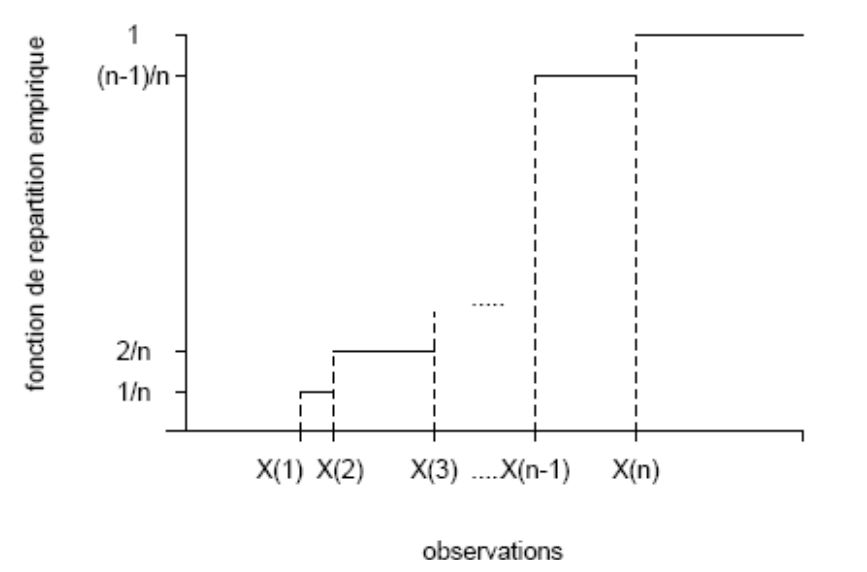
\includegraphics[scale=0.3]{Figures/Fct_de_repartition_empirique}
\end{center}


\paragraph{Remarques}
\begin{enumerate}[label=(\arabic*)]
\item Lorsque $F_n(t) \to F(t)$, alors

\item Puisqu'on a
\begin{align*}
\sum_{i=1}^{n} 1_{[x_i \leq t]} \sim Bin(n,\prob{X \leq t})
\end{align*}
Alors,
\begin{align*}
\esp{F_n(t)}		& = \frac{1}{n} n F(t) \\
	& = F(t) \quad \text{(C'est un estimateur sans biais)} \\
Var \left( F_n(t) \right) & = \frac{1}{n^2}  n F(t) S(t) \\
	& = \frac{F(t) S(t)}{n}	\\
	& \underset{n \to \infty}{=} 0 \\
\end{align*}
\end{enumerate}

\subsection{\textit{Cumulative hazard-rate function}}
On utilise cette fonction pour réussir à estimer la fonction de densité et le \textit{hazard rate} empirique. En effet, puisque la distribution empirique est discrète, on ne peut pas dériver $F_n(x)$ pour obtenir $f_n(x)$ et $h_n(x)$. La fonction de hazard cumulative se définit par
\begin{equation}
H_X(x) = - \ln S_X(x)
\end{equation}

\subsection{Notation à utiliser pour la distribution empirique}
\begin{enumerate}[label=\faAngleRight]
\item \blue{$y_1 < y_2 < ... < y_k$} : les $k$ valeurs uniques qui apparaissent dans l'échantillon de $n$. \textbf{Note : } $k \leq n$.

\item \blue{$s_j$} : nombre de fois que l'observation $y_j$ est observée dans l'échantillon. On a
\begin{align*}
\sum_{j=1}^{k} s_j = 1
\end{align*}

\item \blue{$r_j$} : nombre d'observations qui sont plus grandes ou égales à $y_j$. On a
\begin{align*}
r_j = \sum_{i=j}^{k} s_i
\end{align*}

\item Avec cette nouvelle notation, on peut ré-écrire la fonction de répartition empirique : 
\begin{equation}
F_n(x) = 
\begin{cases}
0						& , x < y \\
1 - \frac{r_j}{n}		& , y_{j-1} \leq x \leq y_j \quad j = 2, ..., k \\
1						& , x \geq y_k \\
\end{cases}
\end{equation}
\end{enumerate}

\subsection{Estimateur de Nelson \r{A}alen}
\label{subsec:nelson-Aalen}
Pour pouvoir estimer la \textit{Cumulative hazard-rate function}, on doit utiliser un estimateur qui se base sur la notation utilisée à la sous-section précédente, soit le \textit{Nelson \r{A}alen estimate} : 
\begin{equation}
\hat{H}(x) = 
\begin{cases}
0		& , x < y_1 \\
\sum_{i=1}^{j-1} \frac{s_i}{r_i}	& , y_{j-1} \leq x \leq y_j \quad j = 2, ..., k \\
\sum_{i=1}^{k} \frac{s_i}{r_i}		& , x \geq y_k \\
\end{cases}
\end{equation}

\section{Distribution empirique avec données groupées}

\subsection{Fonction OGIVE}
\red{\textbf{CETTE MATIÈRE NE SERA PAS TESTÉE À L'EXAMEN intra A2018}}


%% VOIR SECTION 11.3 dans le livre %%
% Grahique de fonction de répartition empirique à insérer ici
Dans certains contextes, on a $n$ données qui sont groupées en intervalles. La fonction OGIVE permet d'interpoler entre 2 points $c_{j-1}$ et $c_{j}$.
% Graphique des c^(i) et des intervalles n à insérer ici %%
\begin{align*}
c_{j-1} 	 \leq x  \leq c_j \\
F_n(c_{j-1})	 \leq F_n(x)	 \leq F_n(c_j) \\
\end{align*}
On peut déterminer la valeur empirique de $F_n(x)$ aux bornes des classes, avec
\begin{align*}
F_n(x) = \frac{\sum_{i=1}^{j} n_i}{n}
\end{align*}
où $n_i$ est le nombre d'observations qui sont entre $c_{j-1}$ et $c_j$. Toutefois, pour les valeurs entre deux bornes $c_0 < c_1 < ... < c_k$, il faut approximer avec la fonction OGIV ci-dessous : 

\begin{equation}
\label{eq:repart-OGIVE}
F_n^{\text{OGIVE}}(x) = \frac{c_j - x}{c_j - c_{j-1}} F_n(c_j -1) + \frac{x - c_{j-1}}{c_j - c_{j-1}} F_n(c_j)
\end{equation}



\paragraph{Remarques}
\begin{enumerate}[label=(\arabic*)]
\item Si $x = c_{j-1}$,
\begin{align*}
F_n(c_{j-1}) = F_n^{\text{OGIVE}}(c_{j-1}) \\
\end{align*}
\item Si $x = c_j$,
\begin{align*}
F_n(c_j) = F_n^{\text{OGIVE}}(c_j)
\end{align*}

\item En dérivant \eqref{eq:repart-OGIVE}, on obtient
\begin{align*}
f_n(x) 	& = \derivee{x} F_x(x) \\
		& = \frac{1}{c_j - c_{j-1}} F_x(c_j) - \frac{1}{c_j - c_{j-1}} F_n(c_{j-1}) \\
		& = \frac{F_n(c_j) - F_n(c_{j-1})}{c_j - c_{j-1}} \\ \numberthis
\end{align*}
\end{enumerate}

\chapter{Estimation de données modifiées}
\section{Point estimation}
\subsection{Définitions importante}
Un vocabulaire spécifique aux données modifiées est utilisé, soit

\begin{tabular}{|>{\bfseries} l |>{\em}l |p{3cm}|}
\hline
Définition	& Terme anglais & Explication \\
\hline	\hline
Tronquée à gauche	& left truncated at $d$ & si la valeur observée est plus basse dque $d$, elle n'est pas enregistrée \\
Tronquée à droite	& right truncated at $u$ & si la valeur observée est plus grande que $u$, elle n'est pas enregistrée \\
Censurée à gauche & left censured at $d$ & si la valeur observée est plus basse que $d$, on indique $d$ dans les données modifiées \\
Censurée à droite & right censored at $u$ & si la valeur observée est plus grande que $u$, on indique $u$ dans les données modifiées \\
\hline
\end{tabular}

\textbf{Note} : Il arrive aussi que les données soient \emph{shifted at $d$}, ce qui veut dire qu'on soustrait $d$ aux données (souvent en présence d'un déductible). 

\subsubsection{Notation}
\begin{enumerate}[label=\faAngleRight]
\item \blue{$y_1 < y_2 < ... < y_k$} : les $k$ valeurs uniques qui apparaissent dans l'échantillon.

\item \blue{$x_j$} : la $j$\up{e} données non-censurée qui apparait dans l'échantillon

\item \blue{$d_j$} : le montant auquel $x_j$ est tronquée. Si il n'y a pas de troncage, alors $d_j = 0$.

\item \blue{$u_j$} : la $j$ \up{e} données censurée qui apparait dans l'échantillon.

\item \blue{$r_j$} : nombre d'observations qui sont plus grandes ou égales à $y_j$ (\emph{risk set})
\begin{align*}
r_j = \text{\# of $x_i$} + \text{\# of $u_i$} - (\text{\# of $d_i$} \geq y_j)
\end{align*}

\item \blue{$s_i$} : nombre de décès au temps $i$.
\end{enumerate}

\subsubsection{Estimateur de Kaplan-Meier}
Cet estimateur est une version modifiée de l'estimateur de Nelson-\r{A}alen vu à la section \ref{subsec:nelson-Aalen}. Avec l'information des données et en utilisant la notation vue à la sous-section précédente, on peut estimer la fonction de survie empirique : 
\begin{equation}
\hat{S}_n(t) =
\begin{cases}
1		& , 0 \leq t < y_1 \\
\prod_{i=1}^{j-1} \left( \frac{r_i - s_i}{r_i} \right) & , y_{j-1} \leq t < y_j \quad j = 2, ..., k \\
\prod_{i=1}^{k} \left( \frac{r_i - s_i}{r_i}  \right) & t \geq y_k \\
\end{cases}
\end{equation}


\section{Espérance, Variance et et intervalle d'estimation}

\subsubsection{Contexte}
On s'intéresse à l'espérance et la variance de la fonction de survie $S_n$, qui suite une binomiale (i.e. $S_n(x) \sim Bin(n, S(x))$. Si on connaissait $S(x)$, on pourrait facilement déduire l'espérance et la variance avec les formules qu'on connaît. Toutefois, puisqu'on cherche souvent à estimer $S(x)$, il faudra aussi estimer l'espérance et la variance.

\hl{Section à compléter}














\end{document}
